% Conceptual DentalExplain anatomy; report figure, not an application component.
% !TeX program = xelatex
\documentclass[12pt]{article}
\usepackage[paperwidth=19cm,paperheight=8.6cm,margin=0.5cm]{geometry}
\usepackage{fontspec}
\setmainfont{Times New Roman}
\usepackage{tikz}
\usepackage{graphicx}
\usetikzlibrary{arrows.meta,shapes.geometric}
\pagestyle{empty}
\begin{document}
\noindent\resizebox{\textwidth}{!}{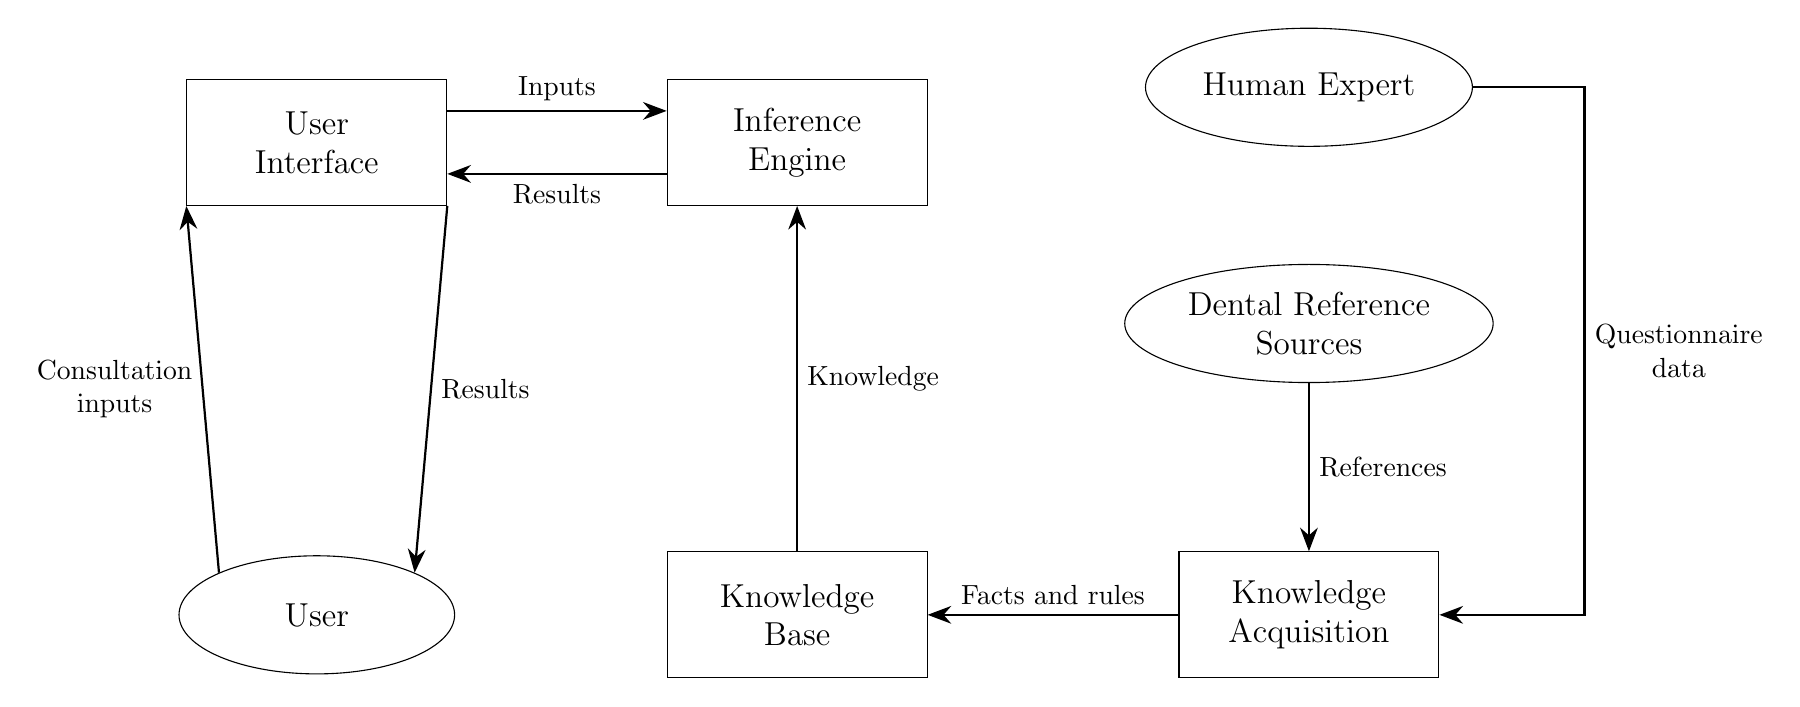
\begin{tikzpicture}[x=1cm,y=1cm,
 component/.style={draw=black,rectangle,minimum width=3.3cm,minimum height=1.6cm,align=center,fill=white},
 person/.style={draw=black,ellipse,minimum width=3.5cm,minimum height=1.5cm,align=center,fill=white},
 flow/.style={-{Stealth[length=3mm]},black,line width=0.8pt},
 every node/.style={font=\large},label/.style={font=\normalsize,align=center}]
\node[component] (ui) at (1.9,8.3) {User\\Interface};
\node[component] (engine) at (8,8.3) {Inference\\Engine};
\node[person] (user) at (1.9,2.3) {User};
\node[component] (kb) at (8,2.3) {Knowledge\\Base};
\node[person] (expert) at (14.5,9) {Human Expert};
\node[person] (sources) at (14.5,6) {Dental Reference\\Sources};
\node[component] (acq) at (14.5,2.3) {Knowledge\\Acquisition};
\draw[flow] (user.north west) -- node[label,left]{Consultation\\inputs} (ui.south west);
\draw[flow] (ui.south east) -- node[label,right]{Results} (user.north east);
\draw[flow] ([yshift=4mm]ui.east) -- node[label,above]{Inputs} ([yshift=4mm]engine.west);
\draw[flow] ([yshift=-4mm]engine.west) -- node[label,below]{Results} ([yshift=-4mm]ui.east);
\draw[flow] (kb.north) -- node[label,right]{Knowledge} (engine.south);
\draw[flow] (expert.east) -- (18,9) -- node[label,right]{Questionnaire\\data} (18,2.3) -- (acq.east);
\draw[flow] (sources.south) -- node[label,right]{References} (acq.north);
\draw[flow] (acq.west) -- node[label,above]{Facts and rules} (kb.east);
\end{tikzpicture}}
\end{document}
